\section{Evaluations}\label{sec:evaluations}
In this section, we comprehensively evaluate the performance of GTenhanced Transformer across various evaluation tasks in our dataset.
% We designed a series of tasks to test various aspects of the model's reconstructive capabilities. Each task addresses different challenges, particularly considering the real-world scenario of missing historical data for certain periods. These tasks serve to benchmark our model against the baseline, ensuring a rigorous evaluation of its effectiveness in reconstructing ancient Chinese pronunciations.

\subsection{Experimental setup}
%\YV{We provide an overview of 5 tasks designed to test various aspects of the model's reconstructive capabilities compared to several baseline models. Each task addresses different challenges, particularly considering the real-world scenario of phonological reconstruction.}
In this subsection, we provide an overview of 5 tasks designed to test various aspects of the model's reconstructive capabilities compared to several baseline models.

\subsubsection{Baselines}
%\HA{This subsection describes several baselines, including random daughter, majority constituent, decision tree, and cognate transformer.}
We compare our model to four baseline models. The random daughter and majority constituent method are from ~\citet{chang_wikihan_2022} but we use an improved version. For each part of the syllable (Initial, Medial, Nucleus and Coda), a random phoneme (random daughter) or a most frequently appearing phoneme(majority constituent) is chosen from inputs of each available historical period and then combined into a syllable as reconstruction result. For decision tree classifier, the reconstruction is also done on each of the four parts. We also adapted cognate transformer~\cite{akavarapu_cognate_2023}, which utilizes both row and column attention to reconstruct the phoneme on each position. Since this model was designed for proto-word reconstruction task where all inputs are contemporary pronunciations, time factor can be embedded but meaningless for our chronological language reconstruction.

% \subsubsection{Evaluation metrics}
% \YV{TBC}
% We use two different kinds of evaluation metrics: edit distance, accuracy and f1 score. For edit distance-based methods, we follow the approach of List, Forkel, et al.(2022), which provides edit distance (ED) and the edit distance normalized by the sequence length (NED). The edit distance is standard Levenshtein distance that penalizes the operation of deletion, insertion or substitution with equal weight of 1. We also provide the edit distance normalized by the syllable length. The F1 score  measures the overall performance of reconstruction.
% We also provide a phoneme-wise comparison method based on articulation similarity. We map a 10-dimension feature vector to each phoneme: the first dimension is used to indicate whether the phoneme is a consonant or not. The next four dimensions(aspirated, voiced, place, method) are all features for consonant. The aspirated and voiced dimensions are binary values, showing the aspiration and voice feature of the phoneme. The place and method dimensions are normalized range of values, indicating 9 places and 8 methods of articulation. The last five dimensions (frontback, updown, dorsal, rounded, rhotic) are for vowels. (frontback, updown) together describes the place of articulation. Dorsal/apical is a special concept in Sino-Tibetan languages, demonstrating a pair of contrastive phonemes. Rounded reflects the shape of the lips during articulation. Rhotic refers to a vowel along with an noticeably or prominently pronounced /r/. After this mapping process, we can easily calculate the cosine similarity between two phonemes. We thus take the average similarity score between the reconstructed syllable and the gold syllable for evaluation. 

\subsubsection{Evaluation Tasks}

In this section, we describe the tasks designed to evaluate the performance of GTenhanced Transformer, each testing different aspects of its reconstructive capabilities.

\paragraph{Random Split Evaluation} The dataset is randomly split into training and testing sets with a 7:3 ratio. Due to substantial incomplete data for the Yuan and MingQing periods, we first partition the dataset into four subsets: characters missing both Yuan and MingQing pronunciations, characters missing only Yuan pronunciations, characters missing only MingQing pronunciations, and characters with no missing data. Each subset is then split into training and testing sets using the same seed for randomization, ensuring a 7:3 ratio. The subsets are then combined to form the final training and testing datasets.

\paragraph{Phonetic Distinction Evaluation} Characters with phonetically same Modern pronunciations are segregated to ensure they do not appear in both the training and testing sets, increasing the difficulty of the task. The dataset is first divided into four subsets as in the Random Split Evaluation, then split into training and testing sets while maintaining phonetic distinction, and finally combined to form the final datasets.

\paragraph{Evaluation with Reduced Training Data from the Reconstructed Era} This task involves decreasing the amount of training data from the reconstructed era. For example, to reconstruct Modern pronunciations, the training set may contain only a fraction of the available Modern data or none at all. The training and testing sets are split as in the Phonetic Distinction Evaluation, ensuring no overlap of phonetically similar characters between sets.

\paragraph{Evaluation with Reduced Historical Training Data} We progressively reduce the historical phonetic data available for training to assess the model's performance under varying levels of data scarcity. For example, to reconstruct Modern pronunciations, we provide data from only the MiddleTang, LateTang, and Song periods, or fewer. The training and testing sets are split as in the Phonetic Distinction Evaluation.

\paragraph{Predict Future Pronunciation} This task predicts possible future pronunciations using the known pronunciations from six historical periods: MiddleTang, LateTang, Song, Yuan, MingQing, and Modern. The model's predictions are purely speculative due to the absence of ground truth data. This exploration offers insights into the model's capacity for extrapolation and generalization beyond historical contexts.

% \subsection{Ablation Studies}
% \YV{TB checked}
% To demonstrate the effectiveness of incorporating glyph features in our transformer-based model, we conducted a series of ablation studies. These studies aimed to isolate the impact of glyph information on the model's performance in reconstructing ancient Chinese pronunciation.

% \paragraph{Experimental Setup}
% We designed the ablation studies by creating two versions of our model:

% Full Model: This version includes all features—phonetic, glyph, and linguistic rules.
% No Glyph Model: This version excludes glyph features, relying solely on phonetic and time inputs.
% Both models were trained and evaluated on the same dataset, ensuring a consistent comparison. We used standard accuracy metrics to assess the performance across normal, hard, and low-resource reconstruction tasks.

\subsection{Experiment Results}

\paragraph{Random Split Evaluation}

\tabref{tab:random split} shows our model's superior performance in reconstructing pronunciations across all historical periods in the random split task. The results shown are averaged over three runs. Despite significant data gaps in the Yuan and MingQing periods, our model consistently achieves an F1 score above 0.85. In contrast, the decision tree model's performance suffers due to extensive missing data during these periods, highlighting our model's robustness in handling incomplete datasets.

Furthermore, compared to the Cognate Transformer model, our approach exhibits a slight advantage in reconstructing pronunciations for the Yuan and MingQing periods. This edge is attributed to our model's ability to effectively integrate glyph and temporal features, enabling a nuanced understanding of phonetic evolution over time and facilitating accurate reconstructions in data-sparse periods.

\begin{table}[ht]
    \centering
    \footnotesize
    \begin{tabular}{l@{\hskip 10pt}c@{\hskip 10pt}c@{\hskip 10pt}c@{\hskip 10pt}c@{\hskip 10pt}c@{\hskip 10pt}c}
    \hline
    \textbf{Model} & \textbf{T} & \textbf{L} & \textbf{S} & \textbf{Y} & \textbf{Q} & \textbf{M}\\
    \hline
    RD & 0.167 & 0.179 & 0.181 & 0.157 & 0.166 & 0.155\\
    MC & 0.175 & 0.179 & 0.196 & 0.194 & 0.207 & 0.219\\
    \hline
    DT & 0.947 & 0.976 & 0.953 & 0.442 & 0.353 & 0.787\\
    CT & 0.958 & 0.965 & 0.923 & 0.810 & 0.838 & 0.867\\
    GTeT & \textbf{0.961} & \textbf{0.980} & \textbf{0.972} & \textbf{0.852} & \textbf{0.873} & \textbf{0.876}\\
    \hline
    \end{tabular}
    \caption{Model performance on random split evaluation (Metrics: F1). Abbreviations: RD - Random Daughter, MC - Majority Constituent, DT - Decision Tree, CT - Cognate Transformer, GTeT - GTenhanced Transformer.}
    \label{tab:random split}
\end{table}

\paragraph{Phonetic Distinction Evaluation}

\tabref{tab:strict split} shows that our model still maintains optimal performance and a high F1 score even under the strict partitioning of the training and testing sets. The results are also averaged over three runs. In this scenario, characters with the same pronunciation do not appear in both the training and testing sets simultaneously. However, by leveraging glyph and temporal features, our model can accurately reconstruct target pronunciations from related phonetic information. This demonstrates the model's ability to generalize and infer pronunciations based on learned patterns, even when direct phonetic similarities are not present in the training data.

\begin{table}[ht]
    \centering
    \footnotesize
    \begin{tabular}{l@{\hskip 10pt}c@{\hskip 10pt}c@{\hskip 10pt}c@{\hskip 10pt}c@{\hskip 10pt}c@{\hskip 10pt}c}
    \hline
    \textbf{Model} & \textbf{T} & \textbf{L} & \textbf{S} & \textbf{Y} & \textbf{Q} & \textbf{M}\\
    \hline
    RD & 0.167 & 0.179 & 0.181 & 0.157 & 0.166 & 0.155\\
    MC & 0.175 & 0.179 & 0.196 & 0.194 & 0.207 & 0.219\\
    \hline
    DT & 0.821 & 0.889 & 0.794 & 0.131 & 0.171 & 0.451\\
    CT & 0.863 & 0.928 & 0.855 & 0.613 & 0.574 & 0.500\\
    GTeT & \textbf{0.931} & \textbf{0.942} & \textbf{0.933} & \textbf{0.702} & \textbf{0.652} & \textbf{0.728}\\
    \hline
    \end{tabular}
    \caption{Model performance on phonetic distinction evaluation (Metrics: F1).}
    %\KZ{Make these two tables narrow tables by using abbrev.}
    \label{tab:strict split}
\end{table}

\paragraph{Evaluation with Reduced Training Data from the Reconstructed Era}

\figref{fig:reduce input data} and \tabref{tab:reduce input data} depict the findings from our Evaluation with Reduced Training Data from the Reconstructed Era. Here, the decision tree model's performance diminishes linearly as training data decreases. In contrast, attention-based models like the Cognate Transformer and our GTenhanced Transformer exhibit a logarithmic decline in performance under reduced training conditions, indicating their resilience to data reduction.

Our GTenhanced Transformer notably maintains a significant F1 score even when no training data for M pronunciations is available. This resilience stems from its ability to leverage character glyph and temporal features, facilitating accurate reconstructions based on related historical data. These results underscore the robustness of our model in handling sparse datasets, highlighting its practical potential where complete data is often lacking.

As shown in \tabref{tab:reduce input data}, both the Decision Tree and Cognate Transformer models exhibit zero performance (F1 score of 0) when there is no training data from the reconstructed era. The Decision Tree model relies on patterns seen during training to make reconstructions, rendering it ineffective without target-era data. Similarly, the Cognate Transformer model's use of row and column attention fails without target-era training, hindering its ability to establish meaningful connections for accurate reconstructions across historical periods.
% For the Decision Tree model, this is expected as it relies on patterns seen during training to make reconstructions; without any data from the target era, it cannot make informed reconstructions. Cognate Transformer model also fails to reconstruct in the absence of target-era training data. This is because the Cognate Transformer model utilizes both row and column attention to reconstruct the phoneme at each position. Without training data from the target era, the model cannot effectively utilize glyph and temporal features to establish attention between known pronunciations and unknown target-era pronunciations. Consequently, it lacks the ability to form meaningful connections and infer phonetic patterns across different periods, resulting in an inability to make accurate reconstructions for the target era.

Moreover, the decline in F1 scores with the reduction of target period data in the training set further validates the effectiveness of our dataset. The dataset's richness in historical and phonetic context is crucial for accurate pronunciation reconstruction, and the model's performance drop with less data underscores this importance.

\begin{figure}[ht]
    \centering
    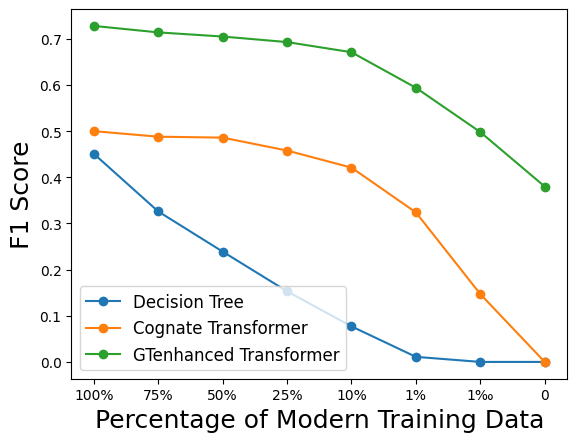
\includegraphics[width=0.35\textwidth]{images/target_reduced.png}
    \caption{Model performance on evaluation with reduced training data from the reconstructed era.}
    \label{fig:reduce input data}
\end{figure}

\begin{table*}[ht]
    \centering
    \footnotesize
    \begin{tabular}{l c c c c c c c c}
    \hline
    \textbf{Model} & \textbf{100\%}  & \textbf{75\%} & \textbf{50\%} & \textbf{25\%} & \textbf{10\%} & \textbf{1\%} & \textbf{1\textperthousand} & 0 \\
    \hline
    Decision Tree & 0.451 & 0.326 & 0.239 & 0.153 & 0.077 & 0.011 & 0 & 0\\
    Cognate Transformer & 0.500 & 0.488 & 0.486 & 0.458 & 0.421 & 0.324 & 0.147 & 0\\
    GTenhanced Transformer & \textbf{0.728} & \textbf{0.714} & \textbf{0.705} & \textbf{0.693} & \textbf{0.671} & \textbf{0.594} & \textbf{0.498} & \textbf{0.380}\\
    \hline
    \end{tabular}
    \caption{Model performance on Reduced Target Training Data Evaluation (Metrics: F1). The target of the model reconstruction is Modern pronunciation. The value of the header represent the percentages of Modern pronunciation data in the training set relative to the entire training set. The division between the training and testing sets follows the phonetic distinction evaluation.}
    %\KZ{Need to explain the zeros in the table.}
    \label{tab:reduce input data}
\end{table*}

\paragraph{Evaluation with Reduced Historical Training Data}

As shown in \figref{fig:reduce history context}, we progressively reduce the historical context data when reconstructing Modern pronunciation. The F1 score decreases more slowly compared to reconstructing MiddleTang pronunciation. Specifically, when reconstructing Modern pronunciation, the F1 score drops from 0.380 to 0.285 as we reduce the available historical context from T+L+S+Y+Q to only T. On the other hand, when reconstructing MiddleTang pronunciation, the F1 score drops from 0.682 to 0.283 as we reduce the historical context from L+S+Y+Q+M to only M. The F1 scores become nearly identical at the final stages. This phenomenon stems from the model's heavier reliance on phonetic information and attention weights from adjacent eras, particularly MiddleTang, LateTang, and Song periods, which exhibit structured and rule-based phonetic patterns.

Additionally, the decline in F1 scores also validates the effectiveness of our dataset. As we reduce the historical context, the model's performance drops, indicating that the available historical phonetic information is crucial for accurate pronunciation reconstruction.

\begin{figure}[ht]
    \centering
    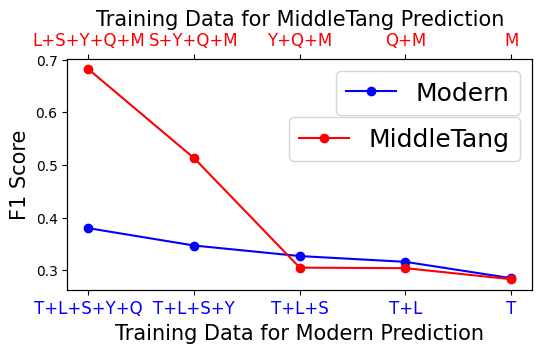
\includegraphics[width=0.35\textwidth]{images/history_reduced.png}
    \caption{Model performance on evaluation with reduced historical training data.}
    \label{fig:reduce history context}
\end{figure}

\paragraph{Predict Future Pronunciations}
Our model has demonstrated robust performance, maintaining a certain level of F1 score even in the absence of training data for specific historical periods. To further explore the capabilities of our model, we conducted an intriguing experiment to predict the pronunciation of Chinese characters in AD 2300\footnote{You can listen to the audio representations of future Chinese pronunciations at the following address: \href{http://47.97.123.246:8080/}{Predict Future Pronunciations Demo}}.
%\href{47.97.123.246:8080}{Future Chinese Pronunciation Demo}